
\vspace{0.15cm}
\begin{flushleft}
	{\color{blue!50!green}\fbox{\fontfamily{qag}\bfseries\selectfont PHẦN I. Câu trắc nghiệm nhiều phương án lựa chọn (3,0 điểm)}}
	\textit{\small (Thí sinh trả lời từ câu 1 đến câu 12. Mỗi câu hỏi thí sinh chỉ chọn một phương án.)}
\end{flushleft}
\setcounter{ex}{0}
\setcounter{bt}{0}

% Câu 1
\begin{ex}
	\macau{ID: VL10-QH104-C01}Một vật chuyển động thẳng có độ dịch chuyển $d_1$ tại thời điểm $t_1$ và độ dịch chuyển $d_2$ tại thời điểm $t_2$. Vận tốc trung bình của vật trong khoảng thời gian từ $t_1$ đến $t_2$ là
	\choice
	{$v_{\text{tb}} = \dfrac{d_1 + d_2}{t_2 - t_1}$}
	{$v_{\text{tb}} = \dfrac{1}{2}\left(\dfrac{d_1}{t_1} + \dfrac{d_2}{t_2}\right)$}
	{$v_{\text{tb}} = \dfrac{d_1 - d_2}{t_1 + t_2}$}
	{\True $v_{\text{tb}} = \dfrac{d_2 - d_1}{t_2 - t_1}$}
	\loigiai{
		Vận tốc trung bình bằng thương số giữa độ dịch chuyển và khoảng thời gian thực hiện độ dịch chuyển đó:\par
		\[v_{\text{tb}} = \frac{\Delta d}{\Delta t} = \frac{d_2 - d_1}{t_2 - t_1}.\]
	}
\end{ex}

% Câu 2
\begin{ex}
	\macau{ID: VL10-QH104-C02}Khi một vật chuyển động thẳng ngược chiều dương thì
	\choice
	{\True quãng đường có giá trị dương, độ dịch chuyển có giá trị âm}
	{quãng đường và độ dịch chuyển đều có giá trị âm}
	{quãng đường và độ dịch chuyển đều có giá trị dương}
	{quãng đường có giá trị âm, độ dịch chuyển có giá trị dương}
	\loigiai{
		Quãng đường $s$ là độ dài cung đường đi được nên luôn nhận giá trị dương ($s > 0$). Khi chuyển động ngược chiều dương, tọa độ giảm dần nên độ dịch chuyển nhận giá trị âm ($d < 0$).\par
	}
\end{ex}

% Câu 3
\begin{ex}
	\macau{ID: VL10-QH104-C03}Chỉ dùng thước đo chiều dài và đồng hồ bấm giây để xác định tốc độ trung bình của một chiếc xe đồ chơi chuyển động thẳng từ $A$ đến $B$. Nhận định nào sau đây là \textbf{sai}?
	\choice
	{\True Có thể đo trực tiếp được tốc độ trung bình của chuyển động}
	{Dùng thước đo quãng đường $s$ là phép đo trực tiếp}
	{Dùng đồng hồ bấm giây đo thời gian $t$ là phép đo trực tiếp}
	{Dùng công thức $v = \dfrac{s}{t}$ tính tốc độ trung bình là phép đo gián tiếp}
	\loigiai{
		Tốc độ trung bình được tính toán thông qua công thức $v = \dfrac{s}{t}$ từ kết quả đo trực tiếp quãng đường và thời gian, do đó đây là phép đo gián tiếp. Nhận định A là sai.\par
	}
\end{ex}

% Câu 4
\begin{ex}
	\macau{ID: VL10-QH104-C04}Cuộc cách mạng công nghiệp lần thứ ba bắt đầu vào những năm 70 của thế kỉ XX gắn liền với những thành tựu nghiên cứu đột phá về
	\choice
	{công nghệ vật liệu nano và Vật lí hạt nhân}
	{Internet toàn cầu, robot và trí tuệ nhân tạo}
	{hiện tượng cảm ứng điện từ và mạng lưới điện xoay chiều}
	{\True điện tử, chất bán dẫn và vi mạch tích hợp}
	\loigiai{
		Cách mạng công nghiệp lần thứ ba (cuối thế kỉ XX) bùng nổ nhờ sự phát triển vượt bậc của chất bán dẫn, vi mạch điện tử và máy tính kĩ thuật số nhằm tự động hóa sản xuất.\par
	}
\end{ex}

% Câu 5
\begin{ex}
	\macau{ID: VL10-QH104-C05}Sai số tỉ đối $\delta A$ của một phép đo đại lượng vật lí là
	\choice
	{tỉ số giữa sai số ngẫu nhiên và sai số hệ thống}
	{tỉ số giữa sai số tuyệt đối và sai số ngẫu nhiên}
	{tỉ số giữa sai số ngẫu nhiên và sai số tuyệt đối}
	{\True tỉ số giữa sai số tuyệt đối và giá trị trung bình của đại lượng cần đo}
	\loigiai{
		Sai số tỉ đối là tỉ số phần trăm giữa sai số tuyệt đối và giá trị trung bình của đại lượng cần đo: $\delta A = \dfrac{\Delta A}{\overline{A}} \cdot 100\%$.\par
	}
\end{ex}

% Câu 6
\begin{ex}
	\macau{ID: VL10-QH104-C06}Trong các hoạt động sau trong phòng thực hành Vật lí: \par (1) Để các chất dễ cháy gần nguồn điện và thí nghiệm mạch điện. \par (2) Bỏ chất thải thí nghiệm đúng nơi quy định. \par (3) Dùng tay không cầm ống chứa hóa chất nguy hiểm. \par (4) Đọc kĩ hướng dẫn sử dụng và quan sát các kí hiệu cảnh báo trên thiết bị. \par (5) Sử dụng trang phục và trang thiết bị bảo hộ phù hợp. \par (6) Thực hiện thao tác nhanh và mạnh bằng mọi giá. \par Những hoạt động đảm bảo an toàn là
	\choice
	{(2), (4), (5), (6)}
	{(1), (2), (4)}
	{\True (2), (4), (5)}
	{(2), (4), (6)}
	\loigiai{
		Các hành động (2), (4), (5) là đúng quy chuẩn an toàn thực hành. Các hành động (1), (3), (6) vi phạm an toàn, có nguy cơ gây cháy nổ, bỏng hoặc hư hại thiết bị.\par
	}
\end{ex}

% Câu 7
\begin{ex}
	\macau{ID: VL10-QH104-C07}Kết luận nào sau đây đúng khi nói về độ dịch chuyển và quãng đường đi được của một vật?
	\choice
	{Độ dịch chuyển và quãng đường đi được đều là đại lượng vectơ}
	{Độ dịch chuyển và quãng đường đi được đều là đại lượng không âm}
	{\True Độ dịch chuyển là đại lượng vectơ, quãng đường đi được là đại lượng vô hướng}
	{Độ dịch chuyển và quãng đường đi được đều là đại lượng vô hướng}
	\loigiai{
		Độ dịch chuyển $\vec{d}$ là đại lượng vectơ nối vị trí đầu và vị trí cuối; quãng đường $s$ là đại lượng vô hướng biểu diễn độ dài quỹ đạo chuyển động.\par
	}
\end{ex}

% Câu 8
\begin{ex}
	\macau{ID: VL10-QH104-C08}Một con thuyền đi dọc theo một dòng sông từ $A$ đến $B$ rồi trở về lại $A$ ($A$ và $B$ cách nhau $24\text{ km}$). Tốc độ của thuyền khi nước đứng yên là $10\text{ km/h}$. Tốc độ dòng nước chảy là $2\text{ km/h}$. Tổng thời gian chuyển động của thuyền cả đi lẫn về là
	\choice
	{\True $5\text{ h}$}
	{$3\text{ h}$}
	{$2\text{ h}$}
	{$8\text{ h}$}
	\loigiai{
		-- Vận tốc khi xuôi dòng: $v_1 = 10 + 2 = 12\text{ km/h} \Rightarrow t_1 = \dfrac{24}{12} = 2\text{ h}$.\par
		-- Vận tốc khi ngược dòng: $v_2 = 10 - 2 = 8\text{ km/h} \Rightarrow t_2 = \dfrac{24}{8} = 3\text{ h}$.\par
		-- Tổng thời gian: $t = t_1 + t_2 = 2 + 3 = 5\text{ h}$.\par
	}
\end{ex}

% Câu 9
\begin{ex}
	\macau{ID: VL10-QH104-C09}Phát biểu nào sau đây đúng khi nói về chuyển động thẳng biến đổi đều?
	\choice
	{Vật chuyển động thẳng đều thì gia tốc luôn luôn khác không}
	{Vật chuyển động thẳng chậm dần đều thì gia tốc luôn luôn có giá trị âm}
	{\True Vật chuyển động thẳng nhanh dần đều theo chiều âm thì gia tốc có giá trị âm}
	{Vật chuyển động thẳng nhanh dần đều thì gia tốc luôn thay đổi theo thời gian}
	\loigiai{
		Khi chuyển động nhanh dần đều theo chiều âm thì $v < 0$ và $a$ cùng dấu với $v$ ($a \cdot v > 0$), do đó gia tốc $a < 0$.\par
	}
\end{ex}

% Câu 10
\begin{ex}
	\macau{ID: VL10-QH104-C10}Đồ thị vận tốc -- thời gian $(v - t)$ nào dưới đây mô tả chuyển động thẳng chậm dần đều theo chiều dương?
	\begin{center}
		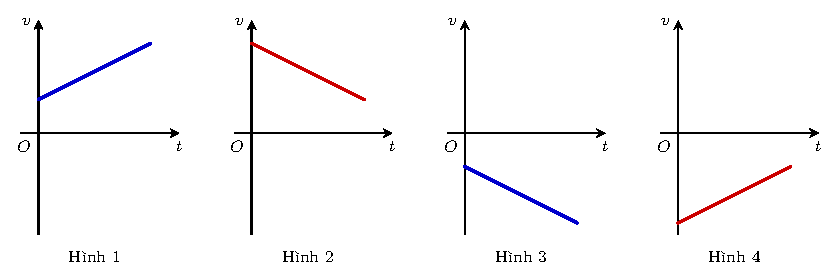
\includegraphics[width=12.0cm]{fig_cau10_vt.pdf}
	\end{center}
	\choice
	{Hình 1 và Hình 2}
	{\True Hình 2}
	{Hình 2 và Hình 4}
	{Hình 3}
	\loigiai{
		Chuyển động thẳng chậm dần đều theo chiều dương có $v > 0$ và độ lớn vận tốc giảm dần theo thời gian, được biểu diễn bởi đường thẳng dốc xuống ở nửa mặt phẳng trên trục hoành (Hình 2).\par
	}
\end{ex}

% Câu 11
\begin{ex}
	\macau{ID: VL10-QH104-C11}Một vật chuyển động thẳng biến đổi đều có phương trình độ dịch chuyển $d = 4t + t^2\text{ (m; s)}$. Phương trình vận tốc của vật theo thời gian là
	\choice
	{$v = 1 + 4t\text{ (m/s)}$}
	{\True $v = 4 + 2t\text{ (m/s)}$}
	{$v = 4 + t\text{ (m/s)}$}
	{$v = 2t\text{ (m/s)}$}
	\loigiai{
		Đối chiếu với phương trình tổng quát $d = v_0 t + \dfrac{1}{2}at^2$:\par
		\[v_0 = 4\text{ m/s}, \quad \frac{1}{2}a = 1 \Rightarrow a = 2\text{ m/s}^2.\]
		Phương trình vận tốc: $v = v_0 + at = 4 + 2t\text{ (m/s)}$.\par
	}
\end{ex}

% Câu 12
\begin{ex}
	\macau{ID: VL10-QH104-C12}Chuyển động của vật nào sau đây trong không khí có thể xem gần đúng là sự rơi tự do?
	\choice
	{Một viên đạn vừa bay ra khỏi nòng súng}
	{\True Một viên đá nhỏ được thả rơi tự do từ trên cao xuống đất}
	{Một chiếc lá bàng đang rơi rụng từ trên cành cây}
	{Một vận động viên đang nhảy dù trong không trung}
	\loigiai{
		Viên đá nhỏ có khối lượng riêng lớn và hình dạng gọn, lực cản của không khí tác dụng lên nó là không đáng kể so với trọng lượng, nên chuyển động gần đúng là sự rơi tự do.\par
	}
\end{ex}

\vspace{0.15cm}
\begin{flushleft}
	{\color{blue!50!green}\fbox{\fontfamily{qag}\bfseries\selectfont PHẦN II. Câu trắc nghiệm đúng sai (2,0 điểm)}}
	\textit{\small (Thí sinh trả lời từ câu 1 đến câu 2. Trong mỗi ý a), b), c), d) ở mỗi câu, thí sinh chọn đúng hoặc sai.)}
\end{flushleft}
\setcounter{ex}{0}
\setcounter{bt}{0}

% Phần II Câu 1
\begin{ex}
	\macau{ID: VL10-QH104-C13}Chuyển động của một vật dọc theo một đường thẳng cố định có đồ thị vận tốc -- thời gian $(v - t)$ như hình bên.
	\begin{center}
		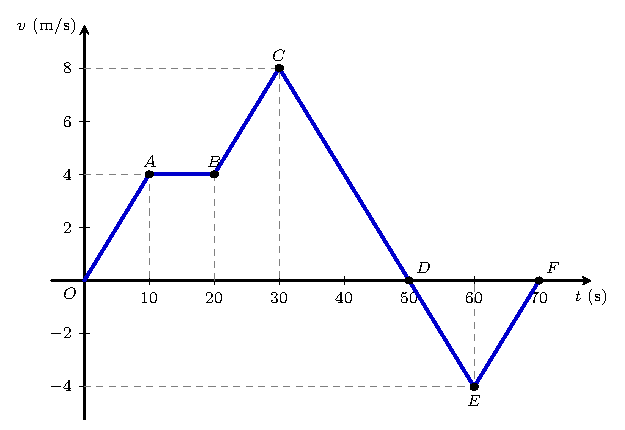
\includegraphics[width=7.0cm]{fig_cau13_vt.pdf}
	\end{center}
	\choiceTF[t]
	{\True Gia tốc của vật trong khoảng thời gian từ giây thứ $60$ đến giây thứ $70$ là $0{,}4\text{ m/s}^2$}
	{Trong suốt khoảng thời gian từ $10\text{ s}$ đến $20\text{ s}$, vật đứng yên không chuyển động}
	{Trong khoảng thời gian từ $30\text{ s}$ đến $50\text{ s}$, vật chuyển động thẳng chậm dần đều theo chiều âm}
	{\True Tổng độ dịch chuyển của vật từ thời điểm $0\text{ s}$ đến giây thứ $70$ bằng $160\text{ m}$}
	\loigiai{
		{\color{green!50!black}\textbf{a) Đúng}} Tại $t = 60\text{ s}$, $v_E = -4\text{ m/s}$; tại $t = 70\text{ s}$, $v_F = 0$. Gia tốc: $a = \dfrac{0 - (-4)}{70 - 60} = 0{,}4\text{ m/s}^2$.\par
		{\color{red!80!black}\textbf{b) Sai}} Từ $10\text{ s}$ đến $20\text{ s}$, đồ thị nằm ngang ở $v = 4\text{ m/s}$, vật chuyển động thẳng đều, không phải đứng yên.\par
		{\color{red!80!black}\textbf{c) Sai}} Từ $30\text{ s}$ đến $50\text{ s}$, đồ thị nằm phía trên trục hoành ($v > 0$) và độ lớn vận tốc giảm dần về $0$, vật chuyển động chậm dần đều theo chiều dương.\par
		{\color{green!50!black}\textbf{d) Đúng}} Độ dịch chuyển bằng hiệu diện tích: phần trên trục hoành $S_1 = \dfrac{1}{2} \cdot 10 \cdot 4 + 10 \cdot 4 + \dfrac{4+8}{2} \cdot 10 + \dfrac{1}{2} \cdot 20 \cdot 8 = 20 + 40 + 60 + 80 = 200\text{ m}$. Phần dưới trục hoành $S_2 = \dfrac{1}{2} \cdot 20 \cdot 4 = 40\text{ m}$. Độ dịch chuyển $d = S_1 - S_2 = 200 - 40 = 160\text{ m}$.\par
	}
\end{ex}

% Phần II Câu 2
\begin{ex}
	\macau{ID: VL10-QH104-C14}Bạn Nam đi xe đạp từ nhà đến trường học hết thời gian $5\text{ phút}$ ($300\text{ s}$) dọc theo trục $Ox$, sau đó quay đầu đi ngược lại siêu thị hết thời gian $2\text{ phút}$ ($120\text{ s}$). Biết khoảng cách từ nhà đến trường là $1\,000\text{ m}$, siêu thị cách trường $200\text{ m}$ và nằm trên đoạn đường nối giữa nhà và trường học như hình bên.
	\begin{center}
		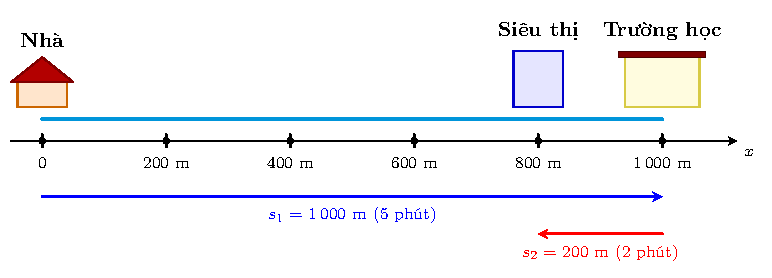
\includegraphics[width=11.5cm]{fig_cau14_nam.pdf}
	\end{center}
	\choiceTF[t]
	{\True Tổng chiều dài quãng đường thực tế mà bạn Nam đã đi bằng $1\,200\text{ m}$}
	{\True Độ lớn vectơ độ dịch chuyển tổng hợp của bạn Nam sau cả hai chặng bằng $800\text{ m}$}
	{Tốc độ trung bình trên toàn bộ hành trình chuyển động của Nam bằng $3{,}3\text{ m/s}$}
	{\True Vận tốc trung bình của Nam trên cả hành trình có độ lớn xấp xỉ bằng $1{,}9\text{ m/s}$}
	\loigiai{
		{\color{green!50!black}\textbf{a) Đúng}} Tổng quãng đường đi được: $s = s_1 + s_2 = 1\,000 + 200 = 1\,200\text{ m}$.\par
		{\color{green!50!black}\textbf{b) Đúng}} Vị trí đầu là nhà ($x = 0$), vị trí cuối là siêu thị ($x = 800\text{ m}$). Độ lớn độ dịch chuyển $d = 800\text{ m}$.\par
		{\color{red!80!black}\textbf{c) Sai}} Tổng thời gian: $\Delta t = 300 + 120 = 420\text{ s}$. Tốc độ trung bình: $v_{\text{tb}} = \dfrac{1\,200}{420} \approx 2{,}86\text{ m/s} \ne 3{,}3\text{ m/s}$.\par
		{\color{green!50!black}\textbf{d) Đúng}} Độ lớn vận tốc trung bình: $v = \dfrac{d}{\Delta t} = \dfrac{800}{420} \approx 1{,}9\text{ m/s}$.\par
	}
\end{ex}

\vspace{0.15cm}
\begin{flushleft}
	{\color{blue!50!green}\fbox{\fontfamily{qag}\bfseries\selectfont PHẦN III. Câu trắc nghiệm trả lời ngắn (2,0 điểm)}}
	\textit{\small (Thí sinh trả lời từ câu 1 đến câu 4.)}
\end{flushleft}
\setcounter{ex}{0}
\setcounter{bt}{0}

% Phần III Câu 1
\begin{ex}
	\macau{ID: VL10-QH104-C15}Một người thợ vô tình làm rơi một chiếc mỏ lết rơi tự do trong giếng thang máy của một tòa nhà cao tầng. Lấy gia tốc trọng trường $g = 9{,}8\text{ m/s}^2$. Sau thời gian $1{,}5\text{ s}$ kể từ lúc rơi, chiếc mỏ lết cách vị trí rơi một khoảng bao nhiêu mét? (Làm tròn kết quả đến hàng đơn vị).

	\par\shortans[oly]{11}
	\loigiai{
		Quãng đường rơi tự do của vật sau thời gian $t = 1{,}5\text{ s}$:\par
		\[s = \frac{1}{2}gt^2 = \frac{1}{2} \cdot 9{,}8 \cdot (1{,}5)^2 = 11{,}025\text{ m} \approx 11\text{ m}.\]
	}
\end{ex}

% Phần III Câu 2
\begin{ex}
	\macau{ID: VL10-QH104-C16}Một máy bay phản lực khi tiếp đất trên đường băng có tốc độ là $100\text{ m/s}$. Biết độ lớn gia tốc hãm cực đại an toàn của máy bay là $5\text{ m/s}^2$. Thời gian ngắn nhất để máy bay có thể dừng hẳn kể từ lúc tiếp đất là bao nhiêu giây?

	\par\shortans[oly]{20}
	\loigiai{
		Vận tốc đầu $v_0 = 100\text{ m/s}$, vận tốc cuối $v = 0$.\par
		Để dừng nhanh nhất, gia tốc hãm có độ lớn cực đại: $a = -5\text{ m/s}^2$.\par
		Thời gian hãm phanh ngắn nhất:\par
		\[t = \frac{v - v_0}{a} = \frac{0 - 100}{-5} = 20\text{ s}.\]
	}
\end{ex}

% Phần III Câu 3
\begin{ex}
	\macau{ID: VL10-QH104-C17}Một hạt electron chuyển động thẳng trong ống phóng điện tử của máy thu hình. Nó được gia tốc đều từ tốc độ đầu $v_0 = 3 \cdot 10^4\text{ m/s}$ đến tốc độ $v = 5 \cdot 10^6\text{ m/s}$ trên đoạn đường dài $2\text{ cm}$. Gia tốc của electron viết dưới dạng $a = X \cdot 10^{14}\text{ m/s}^2$. Tính giá trị của $X$ (làm tròn đến một chữ số thập phân).

	\par\shortans[oly]{6,3}
	\loigiai{
		Đổi quãng đường: $s = 2\text{ cm} = 0{,}02\text{ m}$.\par
		Áp dụng hệ thức độc lập thời gian:\par
		\[v^2 - v_0^2 = 2as \Rightarrow a = \frac{v^2 - v_0^2}{2s} = \frac{(5 \cdot 10^6)^2 - (3 \cdot 10^4)^2}{2 \cdot 0{,}02} \approx \frac{25 \cdot 10^{12}}{0{,}04} = 6{,}25 \cdot 10^{14}\text{ m/s}^2.\]
		Làm tròn đến một chữ số thập phân: $X \approx 6{,}3$.\par
	}
\end{ex}

% Phần III Câu 4
\begin{ex}
	\macau{ID: VL10-QH104-C18}Một học sinh thực hành đo tốc độ chuyển động thẳng đều của một vật. Quãng đường đo được là $s = 19{,}9 \pm 0{,}1\text{ m}$ trong thời gian tương ứng $t = 5{,}0 \pm 0{,}1\text{ s}$. Phép đo tốc độ $v = \dfrac{s}{t}$ có sai số tỉ đối $\delta v$ bằng bao nhiêu phần trăm (\%)? (Làm tròn đến một chữ số thập phân).

	\par\shortans[oly]{2,5}
	\loigiai{
		Sai số tỉ đối của phép đo gián tiếp thương số:\par
		\[\delta v = \delta s + \delta t = \frac{\Delta s}{\overline{s}} \cdot 100\% + \frac{\Delta t}{\overline{t}} \cdot 100\% = \frac{0{,}1}{19{,}9} \cdot 100\% + \frac{0{,}1}{5{,}0} \cdot 100\% \approx 0{,}5\% + 2{,}0\% = 2{,}5\%.\]
	}
\end{ex}

\vspace{0.15cm}
\begin{flushleft}
	{\color{blue!50!green}\fbox{\fontfamily{qag}\bfseries\selectfont PHẦN IV. Tự luận (3,0 điểm)}}
	\textit{\small (Thí sinh trình bày lời giải từ câu 1 đến câu 3.)}
\end{flushleft}
\setcounter{ex}{0}
\setcounter{bt}{0}

% Phần IV Câu 1
\begin{ex}
	\macau{ID: VL10-QH104-C19}Hình bên mô tả đồ thị độ dịch chuyển -- thời gian $(d - t)$ của một người đi xe máy giao hàng chuyển động trên đường thẳng $Ox$.
	\par \textbf{a)} Mô tả trạng thái chuyển động của người đi xe máy trên từng giai đoạn của đồ thị. \par \textbf{b)} Tính tốc độ trung bình và vận tốc của xe máy trong $25\text{ s}$ đầu tiên và trong giai đoạn từ giây thứ $30$ đến giây thứ $45$.
	\begin{center}
		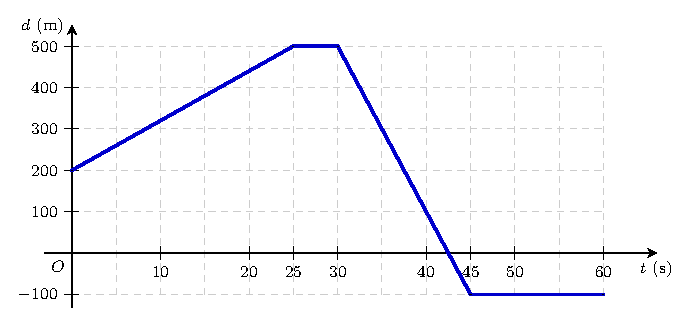
\includegraphics[width=7.5cm]{fig_cau19_shipper.pdf}
	\end{center}
	\loigiai{
		\textbf{a)} Mô tả chuyển động:\par
		-- Từ $0$ đến $25\text{ s}$: Đồ thị là đoạn thẳng dốc lên từ $d = 200\text{ m}$ đến $d = 500\text{ m}$, xe chuyển động thẳng đều theo chiều dương.\par
		-- Từ $25\text{ s}$ đến $30\text{ s}$: Đồ thị nằm ngang ở $d = 500\text{ m}$, xe đứng yên.\par
		-- Từ $30\text{ s}$ đến $45\text{ s}$: Đồ thị là đoạn thẳng dốc xuống từ $d = 500\text{ m}$ về $d = -100\text{ m}$, xe chuyển động thẳng đều ngược chiều dương.\par
		-- Từ $45\text{ s}$ đến $60\text{ s}$: Đồ thị nằm ngang ở $d = -100\text{ m}$, xe đứng yên.\par
		\textbf{b)} Tính toán động học:\par
		-- Trong $25\text{ s}$ đầu tiên (từ $0$ đến $25\text{ s}$): Độ dịch chuyển $\Delta d_1 = 500 - 200 = 300\text{ m}$, quãng đường $s_1 = 300\text{ m}$.\par
		\[v_{\text{tb}1} = \frac{s_1}{\Delta t_1} = \frac{300}{25} = 12\text{ m/s}; \quad v_1 = \frac{\Delta d_1}{\Delta t_1} = \frac{300}{25} = +12\text{ m/s}.\]
		-- Trong giai đoạn từ giây thứ $30$ đến giây thứ $45$ ($\Delta t_2 = 15\text{ s}$): Độ dịch chuyển $\Delta d_2 = -100 - 500 = -600\text{ m}$, quãng đường $s_2 = |\Delta d_2| = 600\text{ m}$.\par
		\[v_{\text{tb}2} = \frac{s_2}{\Delta t_2} = \frac{600}{15} = 40\text{ m/s}; \quad v_2 = \frac{\Delta d_2}{\Delta t_2} = \frac{-600}{15} = -40\text{ m/s}.\]
	}
\end{ex}

% Phần IV Câu 2
\begin{ex}
	\macau{ID: VL10-QH104-C20}Một vật nặng được thả rơi tự do không vận tốc đầu từ đỉnh một ngọn tháp cao xuống đất. Lấy gia tốc trọng trường $g = 9{,}8\text{ m/s}^2$.
	\par \textbf{a)} Tính quãng đường vật rơi được riêng trong giây thứ tư kể từ lúc thả. \par \textbf{b)} Xác định độ tăng vận tốc tức thời của vật trong giây thứ tư đó.
	\loigiai{
		\textbf{a)} Quãng đường vật rơi trong 4 giây đầu: $s(4) = \dfrac{1}{2}g \cdot 4^2 = 8g = 78{,}4\text{ m}$.\par
		Quãng đường vật rơi trong 3 giây đầu: $s(3) = \dfrac{1}{2}g \cdot 3^2 = 4{,}5g = 44{,}1\text{ m}$.\par
		Quãng đường rơi riêng trong giây thứ tư:\par
		\[\Delta s_4 = s(4) - s(3) = 78{,}4 - 44{,}1 = 34{,}3\text{ m}.\]
		\textbf{b)} Độ tăng vận tốc trong giây thứ tư ($\Delta t = 1\text{ s}$):\par
		\[\Delta v = v(4) - v(3) = g \cdot 4 - g \cdot 3 = g = 9{,}8\text{ m/s}.\]
	}
\end{ex}

% Phần IV Câu 3
\begin{ex}
	\macau{ID: VL10-QH104-C21}Cùng một lúc, có hai xe ô tô chuyển động cùng chiều đi qua hai vị trí $A$ và $B$ cách nhau $126\text{ m}$ theo hướng từ $A$ sang $B$. Đồ thị vận tốc -- thời gian $(v - t)$ của hai xe được biểu diễn như hình bên.
	\par \textbf{a)} Xác định gia tốc chuyển động của mỗi xe. \par \textbf{b)} Xác định thời điểm và vị trí hai xe gặp nhau (cách vị trí $A$ bao nhiêu mét)?
	\begin{center}
		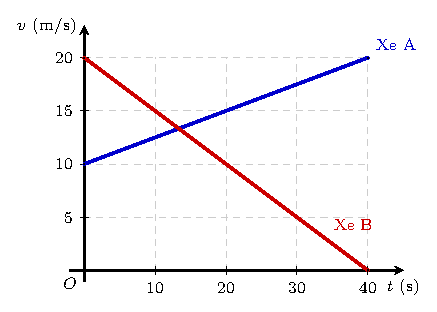
\includegraphics[width=6.8cm]{fig_cau21_haixe.pdf}
	\end{center}
	\loigiai{
		\textbf{a)} Từ đồ thị vận tốc:\par
		-- Xe A: tại $t = 0$ có $v_{0A} = 10\text{ m/s}$; tại $t = 40\text{ s}$ có $v_A = 20\text{ m/s}$. Gia tốc của xe A:\par
		\[a_A = \frac{v_A - v_{0A}}{\Delta t} = \frac{20 - 10}{40} = 0{,}25\text{ m/s}^2.\]
		-- Xe B: tại $t = 0$ có $v_{0B} = 20\text{ m/s}$; tại $t = 40\text{ s}$ có $v_B = 0$. Gia tốc của xe B:\par
		\[a_B = \frac{v_B - v_{0B}}{\Delta t} = \frac{0 - 20}{40} = -0{,}5\text{ m/s}^2.\]
		\textbf{b)} Chọn gốc tọa độ tại $A$, chiều dương từ $A$ sang $B$, gốc thời gian lúc hai xe xuất phát.\par
		Phương trình tọa độ của hai xe:\par
		\[x_A(t) = 10t + \frac{1}{2} \cdot 0{,}25 \cdot t^2 = 10t + 0{,}125t^2\text{ (m)}.\]
		\[x_B(t) = 126 + 20t + \frac{1}{2} \cdot (-0{,}5) \cdot t^2 = 126 + 20t - 0{,}25t^2\text{ (m)}.\]
		Hai xe gặp nhau khi $x_A(t) = x_B(t)$:\par
		\[10t + 0{,}125t^2 = 126 + 20t - 0{,}25t^2 \Leftrightarrow 0{,}375t^2 - 10t - 126 = 0 \Leftrightarrow 3t^2 - 80t - 1\,008 = 0.\]
		Phương trình có $\Delta' = (-40)^2 - 3 \cdot (-1\,008) = 1\,600 + 3\,024 = 4\,624 = 68^2$.\par
		Nghiệm dương hợp lệ:\par
		\[t = \frac{40 + 68}{3} = \frac{108}{3} = 36\text{ s}.\]
		Vị trí hai xe gặp nhau cách mốc $A$ một khoảng:\par
		\[x_A(36) = 10 \cdot 36 + 0{,}125 \cdot 36^2 = 360 + 162 = 522\text{ m}.\]
	}
\end{ex}
